\documentclass[10pt,a4paper]{article}

\usepackage[english]{babel}
\usepackage[utf8]{inputenc}
\usepackage{amsmath}
\usepackage{graphicx}
\usepackage{todonotes}
\usepackage{url}

\title{Extensions on Contract Net Protocol for AGVs \\ \normalsize Multi-agent systems}

\author{Jens Claes \and Victor Le Pochat}

\date{June 3, 2016}

\newcommand{\proposalY}[1]{\todo[inline, color=green]{Proposal (by Yens): #1}}
\newcommand{\proposalV}[1]{\todo[inline, color=green]{Proposal (by Victor): #1}}

\newcommand{\commentY}[1]{\todo[inline, color=yellow]{Yens: #1}}
\newcommand{\commentV}[1]{\todo[inline, color=yellow]{Victor: #1}}

\newcommand{\taskY}[1]{\todo[inline, color=red]{@Yens, fix: #1}}
\newcommand{\taskV}[1]{\todo[inline, color=red]{@Victor, fix: #1}}
\newcommand{\taskS}[1]{\todo[inline, color=red]{@???, fix: #1}}

\newcommand{\MASplot}[2]{
\begin{figure}[htp]
    \centering
    \includegraphics[width=\columnwidth]{#1}
    \caption{#2}
    \label{fig:#1}
\end{figure}
}

\newcommand{\outline}[1]{\todo[inline, caption={}, color=cyan]{\emph{Outline of what should come here}: #1}}

\graphicspath{ {./vpp/}{./images/} }

\begin{document}
\maketitle

\taskS{2 kolommen}

\commentV{Zie https://bitbucket.org/VictorLP/mas/wiki/Notities\commentY{Normaal staan alle comments van de wiki in het verslag nu}}
\section{Introduction}
\outline{Bevat waarom verslag moet lezen (samen met conclusie 1 geheel). The last paragraph of the introduction traditionally says “This report is organised as
follows. Section 1 introduces . . . ”.}
\subsection{Objectives}
The objective of this paper is to investigate whether two extensions of Contract Net (CNET) \cite{CNETStandard,CNET}, namely Contract Net with Confirmation Protocol (CNCP) \cite{CNCP} and Dynamic Contract Net (DynCNET) \cite{DynCNET} are an improvement on CNET itself.

We do this in a drone delivery setting where a company owns a fleet of drones that receives orders from clients, collects the ordered package at one of several warehouses and delivers them to that client. The drones autonomously receive, process and deliver the client orders. The goal is to maximize the company's profit, by having the most suitable drone serve each order. Clients have a time limit for their deliveries, after which the company needs to pay a fine.  Drones can break down and are constrained by their batteries, which can be charged at a warehouse. Drones cannot collide with each other.

We investigate whether any of the aforementioned protocols are suited for a drone company to be profitable in the described setting. We will also check the influence of the number of drones, clients and warehouses on the profit the company can make.
\subsection{Hypotheses}
We formulate the following questions and provide our hypotheses for the answers to them.
\begin{enumerate}
\item \textit{Is there a difference between CNET, CNCP and DynCNET in the profit the company can make?} \\
We expect that the company can make more profit using DynCNET than using CNCP, which should be more profitable than CNET.
\item\textit{Is there a difference in average delivery time between CNET, CNCP and DynCNET?} \\
We expect that CNCP and CNET will deliver faster than DynCNET (as DynCNET wastes time when it switches). We don't expect a difference between CNCP and CNET as both will start delivering quickly and won't waste any time by switching.

\item\textit{Is there a difference in the number of clients that are not delivered between CNET, CNCP and DynCNET?} \\
We expect that CNET and CNCP will deliver the same amount of clients and DynCNET less, again because of the switching between clients.

\item\textit{Is there a difference in the number of messages that needs to be exchanged between CNET, CNCP and DynCNET?}\\
We expect that CNCP will need less messages because we expect less rounds of bidding. CNET will need more messages but still less than DynCNET, which needs a lot of messages due to the dynamism to make sure the best contract is being executed. 

\item\textit{Is it possible to make a profit using any of the 3 approaches?}\\
We expect that all three approaches should be profitable given the right number of warehouses, drones and clients.

\item\textit{What is the influence of the number of drones on the profit?}\\
We expect the profit to scale linearly with the number of drones. Once all clients start to get delivered, saturation will set in.

\item\textit{What is the influence of the number of warehouses on the profit?}\\
We expect the profit to scale with the number of warehouses. As more warehouses become available, it will become more likely to have a warehouse with a low price for the product near the client.

\item\textit{What is the influence of the number of clients on the profit?}\\
We expect the profit to rise until there are too many clients, after which the fines of not delivering start to become too large.
\end{enumerate}

\section{Theory}

In this section we describe the theory of the Contract Net Protocol and the two extensions CNCP and DynCNET. We use the literature on these protocols to highlight their characteristics and differences.

\subsection{Contract Net} The Contract Net Protocol, or CNET, was conceived by Smith in 1980. \cite{CNET} It is a high-level protocol for communication between agents to allow distributed task execution. The high-level protocol messages have a particular structure and meaning, which means the agents can interpret them to receive information on tasks and allocations and to send replies such as bids. 

CNET tries to solve the problem of assigning tasks to idle agents in the most efficient way. Moreover, this problem needs to be solved in a distributed manner, without a central authority that tracks tasks and assigns them with global knowledge.

CNET relies on the negotiation of contracts between a manager and a contractor for the execution of a task. The manager (or initiator) launches a tender for the execution of a task and will monitor the execution and process the results once they arrive. The contractor (or participant) bids on the tenders and when it wins, executes the task and submits the results to the manager. Each agent can be one of these roles for each individual task. This can also mean that an agent acts as a contractor for one task and as a manager for sub-tasks of this task to distribute the workload over several agents.

The Contract Net Protocol is defined by the messages and the information that is contained within them. By having a common language for these messages, all agents can communicate with each other and new agents can immediately start listening for new messages and participate in the negotiation process. There are three types of messages: those related to task announcements, those related to bids and those for the reporting of task results.

A manager initiates the contract negotiation process by adversiting that task with a task announcement message. This message can either be broadcasted to all agents or sent only to one or a few nodes in a focused manner. The task announcement message contains four main parts: an eligibility specification, a task abstraction, a bid specification and an expiration time. The eligibility specification describes what criteria an agent must meet to be able to bid and eventually possibly receive the contract and execute the task. The task abstraction is a description of the task to be executed. The bid specification outlines the expected form of a bid. The expiration time marks the final time at which a bid may be submitted.

Whenever a task announcement arrives at an agent that wants to act as a contractor, all of these parts of the announcement allow contractors to decide whether and when to submit a bid. They add the announcement to a list of received and not expired announcements if they're eligible. The announcements in the list are ranked on interest to the agent. This ranking is a task-specific operation and is based on the information contained within the task announcement.

A busy agent cannot bid while busy, but continues to process the task announcements while executing its task. When this task completes, it can then check the list of task announcements and pick a task to submit a bid on. An idle agent will decide to bid on a task either immediately when it arrives or when it expires. It either submits a bid to the most interesting task or waits for new (better) task anouncements. In a bid, an agent describes its specification in the node abstraction slot. It can also indicate additional information that will be required if the agent may execute the task. Whenever an agent submits a bid to a task, it allocates some resources to that task. This is called early commitment. That agent can then not bid on other tasks at the same moment. This is done to avoid too many task awards to one agent, which would all need to be queued and would slow down the system performance by putting too much load on one agent, which means tasks get executed later.

Bids arrive at the manager and are also ranked and stored in a list until the task can be awarded. The manager can either award a contract immediately if a satisfactory bid arrives (even before the expiration time) or wait for further bids. When the task announcement expires, it can either award the contract to the best bidder in its list or advertise the task again (immediately or after waiting some time). The task is therefore not necessarily awarded when it expires. If a manager awards a contract, it sends a message to the winning contractor, who can start executing the task. When the contractor is finished, it sends a report to the manager with the results of the execution.

The bidding process can be extended to allow agents that cannot or do not want to bid to respond immediately with their reason why they will not bid. Managers can then delay task announcements if no agent is ready to take up the task. An agent can respond immediately if they are ineligible, busy or give the task a low ranking. The manager can then avoid simply reissuing the task announcement when it expires, but can loosen the eligibility requirements if all agents are ineligible or wait before reissuing the task announcement if all agents are busy or not interested yet in the task.

The FIPA version of the Contract Net Protocol \cite{CNETStandard} differs from the original protocol by adding acceptance and rejection of a bid by a manager. This means a contractor is notified if its bid was rejected.

\subsection{Contract Net with Confirmation} 
The Contract Net with Confirmation Protocol, or CNCP, was conceived as an extension to the Contract Net Protocol by Knabe et al. in 2002. \cite{CNCP}

The major shortcoming of CNET that CNCP tries to address is the early commitment by agents. If multiple managers announce a task at the same time, a contractor is only allowed to bid on one of these tasks, after which it already allocates some resources to that task. The agent will choose the task that seems most interesting at that time. The problem is that if a task is somehow very popular, many agents would bid on it but only one would be awarded the task. The other agents then have to wait for the next opportunity to restart the bidding process and try to receive a task. Furthermore the agent has allocated some resources to that popular task, which possibly are only freed after the task announcement expires. This means the agent has less available resources to bid on other tasks later on.

To resolve this issue, in the CNCP the full commitment to a task is moved to the awarding phase: if a contractor is awarded a task, only then does it allocate its resources and stop bidding on other tasks. While a bid has been submitted but the task has not been awarded yet, the contractor can continue bidding on other tasks. When a manager wants to award a task to a contractor, it first contacts that contractor with the request to accept the task. This contractor may however already been awarded a different task, in which case it will refuse the task. The manager may then try to award the task the next best contractor. This either continues until a contractor accepts the task, in which case the contractor can start executing the task and the manager can send a rejection message to the other bidders, or if no contractor accepts it, the manager can announce the task again (possibly after waiting some time).

CNCP requires two more messages to allocate a task: one to request the execution of a task by the manager and one reply to this message by the contractor. If the first contacter bidder refuses, the next best bidder has to be tried and two messages need to be sent. In the worst case this means 2$n$ extra messages (with $n$ the number of bidders) must be sent.

\subsection{Dynamic Contract Net}
The Dynamic Contract Net Protocol, or DynCNET, was conceived as an extension to the Contract Net Protocol by Weyns et al in 2007. \cite{DynCNET}

DynCNET tries to improve on CNET by adding dynamism to the allocation and execution of tasks. More specifically, it addresses the fact that an agent usually has to do some preparation when it is assigned a task before it can actually start executing this task. DynCNET allows contracts to be switched during this preparation phase.

DynCNET changes the acceptance of task by a winning contractor to a provisional acceptance. This means that until further notice that contractor will execute the task and report the results. The contractor can then start its preparation for the execution of the task. During this preparation phase however, the contractor is free to continue bidding on other (new) tasks and the manager may continue announcing the task. If either receives an offer that they consider better than the current contract, they are allowed to cancel the current contract and pursue another task. As soon as a contractor finishes its preparation and starts the actual execution of the task, the contract is final. The contractor is fully committed to the task and no longer bids on other tasks. The contractor also notifies the manager that it is executing the task, which means the manager stops announcing the task.

The synchronization between managers and contractor to assess their current state requires some additional messaging. If a manager cancels a contract, it needs to notify the original contractor that the task has been awarded to another agent. Inversely, a contractor that takes up another task needs to notify the manager of the original task that it is no longer committed to executing that original task. Finally the contractor needs to send a message to the manager when it starts executing the task, so the manager can stop announcing the task to other agents.

\subsection{Alternative Contract Net Protocols}
\taskV{nalezen}
\commentY{\cite{TentativeBidding}, \cite{LeveledCommitment}, \cite{CNETIterativeStandard}, zie ook \cite{DynCNET} Related work voor korte beschrijving}
\commentV{misschien bij theory gedeelte?\commentY{Wat bij theorie gedeelte?}}

\taskS{Nu altijd geschreven als client-drone, aanpassen naar initiator-participant, om te matchen met theorie sectie + eventueel eens kijken dat zelfde termen gebruikt worden}

In the literature, other extensions of CNET can be found. \cite{TentativeBidding} describes a 2-phase protocol (PreBidding and DefinitiveBidding). The first round of pre-bidding is only tentative. The client informs the drones of the tentative results. Drones can still change their offers based on this tentative results and how the world (and other bidding processes) evolve. Once a drone has been tentatively accepted, it can send a definitive bid to the client. If this bid is still better than all tentative bids from other drones, the drone will be informed and both agents commit to the contract. All other drones will be informed that the bidding is definitely over. If the definitive bid is not the best bid, the drone gets tentatively or definitely declined. In case of the former, it can submit a new tentative bid. This protocol can be seen as an extension on CNCP. Drones who get accepted, can accept or decline by choosing the appropriate definitive bid. The advantage of this protocol is that drones who get rejected can still improve their bid.

\cite{CNETIterativeStandard} describes a similar protocol: iterated contract net (ICN). When a client receives bids, it can choose to accept one, or choose to iterate the process by issuing an adapted the call for proposal to a subset of the bidders. The intent of this next iteration is to receive better bids. The protocol stops when a drone is awarded the contract, the client stops issuing calls for proposals (because all bids are unsatisfactory) or all drones stop bidding.

The tentative bidding of \cite{TentativeBidding} and ICN are very similar. Both protocols can be mapped onto each other.\commentY{Dat erin laten van het mappen op elkaar? Ik denk dat dat het geval is, als ik diagrammen vergelijk, maar niet 100\% zeker} One of the main differences is that ICN issues new calls for proposals and can thus actively try to increase the price of the contract.  In our setting however, both protocols do not make much sense. Drones bid using the estimated profit. They cannot increase their bid, unless the estimated profit changes.

\cite{LeveledCommitment} uses game theory to proof that leveled commitment is to be preferred in all situations over full commitment. In the negotiation of a contract, a decommitting penalty is agreed upon. (This penalty might be different for both agents). When an agent wants to cancel the contract, he has to pay his decommitting fee to the other agent. This not only gives a way to calculate whether or not to cancel a contract in favor of another contract\footnote{They prove (again using game theory) that it is harder than just checking if the profit of the new contract is higher than the fee, because the other agent might decommit if this agent doesn't decommit.}. It also allows contracts that were not possible using full commitment: it is possible that the benefit from a contract is lower than the expected benefit from other contracts that have not yet been announced. But by having the right decommitting fees, a leveled commitment contract might still be interesting for both parties.

It is important to note, that in our design, bids are satisfactory if the expected profit is above the fine for not delivering to this client. (It does not take into account that new clients or drones might become available). The agents described in \cite{LeveledCommitment} take the expected profit of new clients or busy drones into account.

\section{Multi-agent system design}
\outline{Wat wij concreet doen}
\subsection{Design}
We consider a logistics problem where a company serves an area with a fleet of drones. In this area, a number of clients appear with an order for a specific product. One of the drones takes up the order and is dispatched to a warehouse to collect a package with that product. Finally it flies to the client to deliver the package. The goal is to maximize the profit earned on making these deliveries.

Across the world several warehouses are located. For simplification, these warehouses have an infinite stock of every package that a client could potentially order. Drones can pick up packages at these warehouses for a price that varies per warehouse in a range of 80 to 120\% of that package's market price.

Drones can unexpectedly crash and fail. The drone is then written off and the cost of a drone is subtracted from the profit. Drones are also constrained by their batteries, they only have a limited range before they need to charge. Whenever the battery level gets very low, the chances of crashes increase, as the power that comes from the batteries becomes less and less stable. Drones can charge their batteries at the warehouses for a certain cost. They will intelligently choose a route when delivering a package to try as much as possible to avoid having a low battery.

A client has only one order and when that order is delivered, the client stops participating. Client with multiple orders can be reduced to this model by creating multiple clients with one order each. The order consists of the type of package a client wants, the end time by which it wants to have received the package, the price it is willing to pay and the fine it levies if the package is not delivered before the end time. The price and the fine vary around the market price. There are both clients that are initially present in the world and clients that appear randomly afterwards.

For simplification, all agents are completely aware of the whole world and can send messages to all other agents. 

The failures of drones are based on a Poisson distribution and are used in calculating the bid that drones will make on tasks. The bid is based on the estimated minimal cost for a drone to serve the client. The estimated cost consists of four parts: the cost to buy the package from a warehouse; the cost of charging for the battery drain caused by moving between the drone's current location, the warehouse, the client and back to a warehouse to charge; the probabilistic cost of a drone failure on that trajectory; and the price the client is willing to pay (which is subtracted from the other costs). The drone will decide for which warehouse this combined cost is the lowest and submit that as its bid, on the condition that the cost is lower than the fine (then it would just be better not to bother delivering), that it can reach with some battery power left and that it can deliver before the end time of the order.



\commentY{Warehouses randomly algorithm beschrijven}

\outline{\begin{itemize}
        \item drones leveren orders uit warehouses aan clients (1 order per client)
        \item bid berekening (statistisch relevant)
        \item messaging gedetailleerd bespreken of niet?
        \item tijd tijdens opladen wordt niet meegerekend bij estimated cost (footnote)
    \end{itemize}}

\commentY{Add sequence diagrams of 3 protocols??? \commentV{als er nog plaats is in het verslag...}}

\commentV{Agent architecture: zie section 2.3 https://lirias.kuleuven.be/bitstream/123456789/156687/1/CW478.pdf\commentY{Dat is toch veel complexer dan hoe onze architectuur eruit ziet?}}
\subsubsection{Agent state machines}
Both the drone and client use finite state machines to define in which phase of the negotiation they are situated.

\begin{figure}[htp]
    \centering
    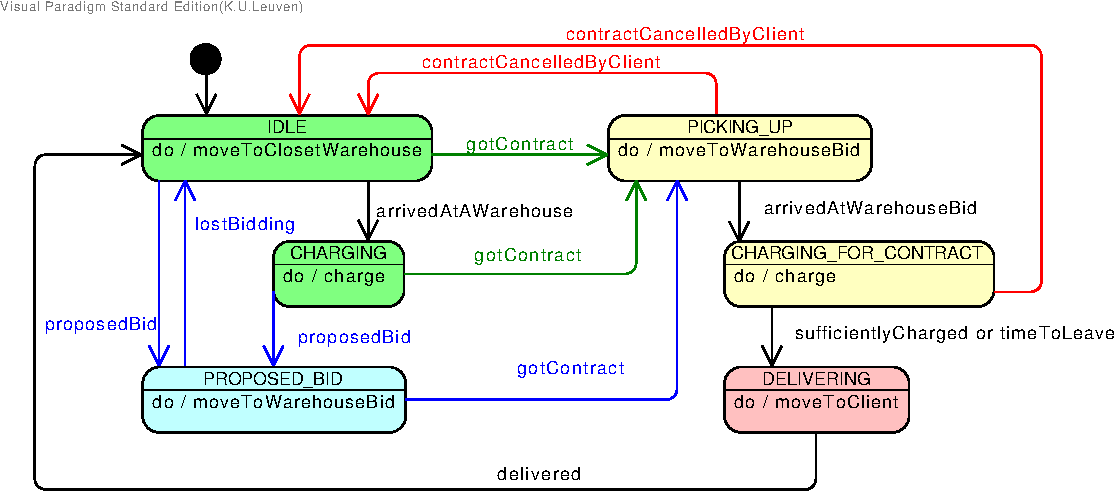
\includegraphics[width=\columnwidth]{Drone}
    \caption{A finite state machine of the drone agent. The blue transitions and state only apply to CNET, the red transitions only to DynCNET and the green transitions to CNCP and DynCNET.}
    \label{fig:droneFSM}
\end{figure}

Figure~\ref{fig:droneFSM} shows the FSM for the drone agent in the three different protocols\footnote{Not represented in the figure is the failed state, in case the drone crashes. A drone can enter this state from all other states and can never leave it again}. The drone starts in the \texttt{IDLE} state. In this state, it will move to the closest warehouse, where it will enter the \texttt{CHARGING} state and start charging. In CNET and CNCP, a drone can bid in the green states. In DynCNET, a drone can bid in the green and yellow states. In CNET, a drone will enter the \texttt{PROPOSED\_BID} state once it has submitted a bid. It will reenter the \texttt{IDLE} state if the client declines. In CNCP and DynCNET, the drone stays in either \texttt{IDLE} or \texttt{CHARGING} and may continue bidding.

If the client awards the task to the drone, the drone goes into the \texttt{PICKING\_UP} state. There it will start moving to the warehouse for which the estimated cost was the lowest. When it gets there, it will go to the \texttt{CHARGING\_FOR\_CONTRACT} state and start charging until either it is sufficiently charged or until it is time to leave due to the client's delivery deadline. In DynCNET, the drone may continue bidding in the \texttt{PICKING\_UP} and \texttt{CHARGING\_FOR\_CONTRACT} states. If it wins another contract, it will stay in or go to the \texttt{PICKING\_UP} state. When the drone leaves, it will pick up the package from the warehouse and enter the \texttt{DELIVERING} state. From then on, it will keep flying to the client until it has arrived, upon which it will deliver the package to the client and enter the \texttt{IDLE} state, thereby moving to the closest warehouse.

The \texttt{PROPOSED\_BID} state is only used in CNET, not in CNCP nor DynCNET.  DynCNET also has two extra transitions: from \texttt{PICKING\_UP} and \texttt{CHARGING\_FOR\_CONTRACT} back to \texttt{IDLE}, in case the client cancels the contract. CNCP and DynCNET also have a direct \texttt{gotContract} transition from \texttt{IDLE} and \texttt{CHARGING\_FOR\_CONTRACT} to \texttt{PICKING\_UP}. In CNET the drone first has to pass through the \texttt{PROPOSED\_BID} state.

\commentY{Ook "biedingen" beter op FSM weergeven? Of dat laten voor sequence diagram\commentY{Ik denk dat sequence diagrammen niet nodig zijn, tenzij we ze in theorie sectie zouden willen zetten.}}

\begin{figure}[htp]
    \centering
    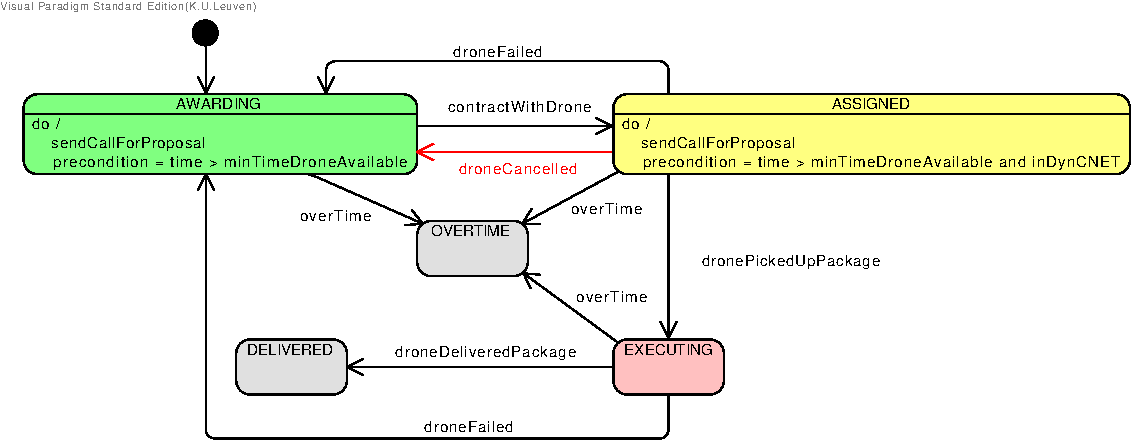
\includegraphics[width=\columnwidth]{Client}
    \caption{A finite state machine of the client agent (the red transition only applies to DynCNET)}
    \label{fig:clientFSM}
\end{figure}

Figure~\ref{fig:clientFSM} shows the FSM for the client agent in the three different protocols. The client starts in the \texttt{AWARDING} state. When the task has been awarded, it enters the \texttt{ASSIGNED} state. From then on, the client will go to the \texttt{EXECUTING} and \texttt{DELIVERED} state respectively when the drone picks up and delivers the package. Only a drone failure or the cancellation of a contract in DynCNET can change the state flow, by having the client return to the \texttt{AWARDING} state. If the maximum delivery time for the client has passed before a drone delivered the package, the client will enter the (final) \texttt{OVERTIME} state.

In CNET and CNCP, a client can only send task announcements while in the \texttt{AWARDING} state. In DynCNET, it can also send task announcements in the \texttt{ASSIGNED} state, until the package is picked up by the drone and the client enters the \texttt{EXECUTING} state.

\commentY{Table met communication primitives as in \cite{TentativeBidding}? \commentV{als er nog plaats is in het verslag...}}

    
\proposalY{
\commentY{Message loss?}

\commentY{Synchronization van DynCNET: }
\commentV{This latter then sends a message to confirm the abort.
moeten we verbreken contract bevestigen? zie DynCNET + CW566: 3.3. Synchronization of abort messages}
}


\subsection{Comparison with existing MAS from literature}
When clients enter the world, they will act as managers and broadcast their task announcement to all agents.\footnote{This includes other clients, who will ignore all task announcements. RinSim does not (yet) provide a broadcast to a subset of all agents, in this case the drones.} This task announcement consists only of the order that a client has. All drones are considered to be eligible. As there is only one type of bid, the bid specification defined in CNET is implicit and left out of the task announcement. There is no separate expiration time for bidding: drones are expected to bid immediately and the task announcement will be sent at the latest on the end time of the order. 

In CNET, only one bid per opportunity (tick) is allowed, so the drone bids on the task for which its cost is the lowest of all received task announcements. Afterwards the drone is committed to that task and cannot bid on other tasks until it is either awarded the task and execution is complete, or until the client explicitly refuses the bid. In the original CNET protocol, a drone would be allowed to bid again at the next tick. Although \cite{CNET} suggests that this might cause significant delays in the system, due to the fact that tasks do not have a bidding expiration time, that clients immediately award contracts if possible and that drones only have one resource, i.e. they can only serve one client at a time, we feel that it does not have as significant an effect. In CNCP and DynCNET, the drone bids on every incoming task while it is not committed to a contract.

The extension where drones that do not bid can respond with their reason is also supported. If a drone has no warehouse for which they can deliver the package for a cost below the fine, they declare themselves as ineligible. If a drone is delivering a package, it answers that it is busy. If in CNET there is a valid bid for a task but it is not the lowest cost of all task announcements, it replies that it has given the task a low ranking.

\cite{CNET} suggests that drones could declare when they are available and what kind of tasks they can execute, so clients can send proposals to award a task directly to an eligible drone. We have decided to instead add a timestamp to the message that the drone is busy, which is a lower limit of when the drone might become available again, based solely on the current distance to the client and not taking the distance to and from warehouses into account. The client can use this information to delay task announcements if no drone is available or interested. More specifically, if all drones are busy or ineligible, the minimum of all estimated times when drones could become available again is taken as the next time for the task announcement. This reduces the number of messages that are sent by the client (and replies by the drones). If a drone gives the task a low ranking, the task announcement is immediately retried as other more interesting tasks will have been awarded and the remaining drones may now rank this task as the best.

A client waits one tick for bids to arrive. All bids are satisfactory, as drones only bid on tasks that are economically viable. The task is then awarded to the best bidder, i.e. the drone with lowest cost. It informs the winning drone that they may start executing the task, and notifies the other bidding drones that their bid has been refused. In CNET, this means the drone can start bidding on other tasks again. Bids that would somehow arrive later will also be refused by the client.

In CNCP and DynCNET, drones can submit multiple bids at the same time and could potentially be awarded multiple tasks. The drone then chooses the task with the lowest cost, notifies the client and starts executing it. It denies all other task assignments and notifies those clients. The tasks are not queued, but released for other drones to fulfil, as delivery takes too long for queueing to be sensible. Clients whose assignments have been denied will reannounce the task instead of trying the next best bidder as in CNCP, as chances are high that due to the short time between announcements and bidding, this next best bidder has already been assigned another task. \commentY{Disagree: note van dat dit een ACL-refuse message is? of via diagram?}  While the original CNCP therefore requires $O(2*n)$ more messages, our design only requires one extra message per bidding round. The number of bidding rounds and therefore the total message count is reduced.

Once a drone has received a task, it starts executing the task by flying to the warehouse with the lowest estimated cost (that was calculated when bidding). It picks up the package at the warehouse and can possibly charge its battery there to make sure that it can complete the delivery, either until it must leave or until the battery is sufficiently charged to minimize the risk of failure. It then flies to the client, delivers the package and flies to the closest warehouse to charge and wait for new tasks. The client is sent a message when the package is picked up and when it is delivered.

In case the drone would crash, the notification of this failure to the client is modeled by sending one last signal to the client. In practice, outside a simulator, a polling approach might be used. After the client is aware of the failure, the client announces the task again.

A potential risk of DynCNET is oscillation of tasks between drones. \cite{DynCNET} describes a solution by limiting the areas of interest, e.g. by broadcasting task announcement only within a limited range. In our design, the agents are limited only by their battery, but not in a communications range. We did not take any special action to prevent the oscillation of tasks between drones.
\outline{
    \begin{itemize}
        \item warehouses oneindige capaciteit
        \item tasks uit literature zijn orders bij ons
        \item verschillen in messaging
        \item concretere berekening bid
        \item Feit dat ze enkel kunnen opladen als ze IDLE (CHARGING) zijn of in CHARGING\_FOR\_WAREHOUSE? En dus niet in andere warehouses. En ook niet voor ze naar andere warehouse vertrekken.
    \end{itemize}
    }
    \commentV{hier zetten? \proposalY{In \cite{CNCP} they first sent a \texttt{Request} message and only upon the \texttt{Agree} message of the client, the \texttt{AcceptProposal} is sent. These two messages from the client to the drone are merged together in our design }}


\section{Experiments}
\subsection{Setup}
\outline{\begin{itemize}
        \item independent: aantal drones, warehouses, clients
        \item dependent: profit, aantal clients delivered, aantal messages, delivery time, ... (\texttt{ExperimentResult})
        \item other: battery drain, kost pakketjes, oplaadkost, ... (\texttt{Variables.kt} + \texttt{PackageType.kt})
        \item beschrijving computer + RinSim 4.1.0
        \item  square area of 100 km$^2$
    \end{itemize}}
\taskS{Experiment 1 en experiment 2!}
\subsection{Results}
\commentY{Een deel van de figuren naar appendix verplaatsen?}
Figures \taskY{nummers} show the results of our experiments. The error-bars represent the 95\%-confidence interval.

\MASplot{drones-profit}{The influence of the number of drones on the profit}
\MASplot{warehouses-profit}{The influence of the number of warehouses on the profit}
\MASplot{initialclients-profit}{The influence of the number of clients at the start of the simulation on the profit}
\MASplot{dynamicclients-profit}{The influence of the number of clients that appear after the start of the simulation on the profit}
\MASplot{dynamicclients-profit-largeNbDrones}{The influence of the number of clients that appear after the start of the simulation on the profit, with a large number of drones}

\MASplot{drones-deliverytime}{The influence of the number of drones on the delivery time}\commentY{omzetten naar seconden ipv milliseconden?}
\MASplot{dynamicclients-delivered-grid2}{The influence of the number of clients that appear after the start of the simulation on the number of clients that are not delivered (in the second experiment) }
\MASplot{dynamicclients-profit-grid2}{The influence of the number of clients that appear after the start of the simulation on the profit (in the second experiment)}


\subsection{Analysis}
\commentY{Echte analyse doen of ook echt expliciet vergelijken met onze hypothese?}
\commentY{In volgorde van de research questions laten of herordenen?}
To test our hypotheses, we used the Games-Howell\taskY{referentie} test. As the data is heteroscedastic, the TukeyHSD-method will have too many Type-I errors.\taskY{Referentie Hubert}. \taskY{referentie} showed that Games-Howell is also robust with non-normal data, which is the case with some of our results. A significance level of 95\% was used for all tests.

Figure~\ref{fig:drones-profit} makes it clear that the number of Drones has an influence on which protocol maximizes profit. In case there are many drones (7 or more), DynCNET is better than CNCP, which outperforms CNET. For an average number of drones (4 to 6), CNCP outperforms CNET and DynCNET. For 3 drones or less, there is no difference between CNET and CNCP, but both outperform DynCNET. As figure~\ref{fig:dynamicclients-profit} and \ref{fig:dynamicclients-profit-largeNbDrones} show, no breakdown happens when enough drones are present. This explains the different relative performance of DynCNET depending on the number of drones.

Figure~\ref{fig:drones-deliverytime} shows the influence of the number of drones on the delivery time. For 1 Drone, DynCNET delivers fastest. There is no significant difference between CNET and CNCP\footnote{in case of 1 drone, both protocols don't differ much}. If 2 or more drones are present in the world, CNCP will deliver faster than CNET, which will deliver faster than DynCNET.

The influence of the protocol on the number of clients that don't get delivered also depend on the number of clients and the number of drones. For a smaller number of clients (less than 20 clients initially and less than 50 clients after the start) or a large number of drones (10 drones), CNCP delivers the most, followed by CNET and DynCNET. In case of 9 drones, no significant difference was found between CNET and DynCNET. In case of 8 drones, DynCNET outperforms CNET. For a smaller number of drones (4 drones), CNET outperforms DynCNET again. Finally, for a very small number of drones (1 or 2 drones), no significant difference was found between CNET and CNCP. In our first experiment, CNCP always outperformed DynCNET. However, figure~\ref{fig:dynamicclients-delivered-grid2} shows that when the number of clients increases, DynCNET starts to outperform CNCP. No region was found, in neither experiment, where CNET outperforms CNCP. Only with 1 or 2 drones in the world, does CNET keep up with CNCP. In that case, both protocols act very similarly anyways.

When there are little number of clients (5 initial clients and 10 extra clients), no significant difference in the number of exchanged messages could be found between CNET and CNCP. However, in general, CNCP needs more messages than CNET. DynCNET always needs more messages than the other two protocols.

As figure~\ref{fig:drones-profit} to \ref{fig:dynamicclients-profit} show, a company can make a profit using any of the three protocols, given the right number of drones and warehouses for the given number of clients in the world.

When increasing the number of drones, the profit increases as well until enough drones are present in the world and saturation is achieved. As saturation sets in quickly in our experiment, no linear region could be found.

When increasing the number of warehouses, the profit increases as well. Figure~\ref{fig:warehouses-profit} shows that this increase seems to slow down as the number of warehouses is further increased. But more experiments would have to be conducted to test this hypothesis. 

When increasing the number of clients (figure~\ref{fig:dynamicclients-profit-grid2}), the profit first increases as well. When the number of clients increases further, the number of clients that aren't delivered increases as well (figure~\ref{fig:dynamicclients-delivered-grid2}). Therefore the profit starts to fall, as the extra fines start to dominate the extra profits. DynCNET outperforms CNET and CNCP in the number of clients that get delivered when increasing the number of clients. Still, in terms of profit, the fall is way steeper. This can be explained using the number of times a drone switches client after being awarded the contract. This number increases linearly with the number of clients up to an average of 15 switches per drone when 200 clients appear after the start of the simulation.

\commentY{Reference Statistische modellen en data-analyse boek van Mia Hubert voor onze statischische methodologie}
\taskS{Reference voor Games-Howell statistische test. \proposalY{http://stats.stackexchange.com/questions/38207/what-are-the-assumptions-of-the-games-howell-multiple-comparisons-procedure, Games, P. A., Keselman, H. J., \& Clinch, J. J. Tests for homogeneity of variance in factorial designs. Psychological Bulletin, 86, 978-984, maar kan hem niet vinden}}

\section{Conclusion}
\commentV{CW566: TABLE 1: INTERFACE DEFINITIONS FOR A TRANSPORT AGENT AND AN AGV AGENT
nakijken of we die allemaal hebben}
\commentY{Ook http://www.fipa.org/specs/fipa00037/SC00037J.html als referentie voor de ACL acts?}
\bibliographystyle{plain}
\bibliography{report}

\end{document}